\documentclass{article}
\usepackage[utf8]{inputenc}
\usepackage{graphicx}
\usepackage{multicol}
\usepackage{caption}
\usepackage{subcaption}
\usepackage{wrapfig}
\usepackage{float}
\usepackage{arydshln}
\usepackage{amsmath,amsthm,amssymb,amsfonts}
\usepackage{hyperref}
\usepackage{makecell}
\usepackage{listings}
\usepackage{epsfig}
\usepackage{color}
\usepackage{natbib}
\usepackage[table]{xcolor}
\usepackage[margin=1.1in]{geometry}
\usepackage[affil-it]{authblk}
\newtheorem{theorem}{Theorem}
\newtheorem{lemma}{Lemma}



\def\T{{\mathrm{\scriptscriptstyle T}}}
\def\bmath#1{\mbox{\boldmath$#1$}}

\bibpunct{(}{)}{;}{a}{}{,}
\setlength{\bibsep}{4.0pt}
\renewcommand{\baselinestretch}{1.1}


\title{\textbf{Analysis of Job Influence on Boise House Prices}}

\author{\vspace{11pt}Bridgette Delight}

\affil[1]{Department of Mathematics, Boise State University, Boise, Idaho 83725}
\affil[2]{Department of Computer Science, Boise State University, Boise, Idaho 83725}

\date{\today}


%------------------------------------------------------------------------------%
\begin{document}
%------------------------------------------------------------------------------%

\maketitle

\begin{abstract}

\end{abstract}

\vspace{8pt}
\noindent
KEY WORDS: Key word one; Key word two; Key word three; Key word four.

\section{Introduction}
Over the past eight years, home prices in the Boise metro area have increased very rapidly, outpacing even some of the largest real estate markets in the country. I was interested in seeing what factors might be influencing this rise, and decided to investigate changes in the Boise Metro Area job market to see if changes in employment types could be leading to the rise in prices. This paper will be comparing changes in Tax Assessed Values (TAV) from 2000-2018 with the changes in Employment by sector over the same time period. 

Earlier this year, the Brookings Institution published a study on employment growth across the nation, and used Boise as one of the case studies. Their analysis highlighted some of the areas where Boise's employment opportunities are growing, as well as the ones that are shrinking. I will use this data as a starting point to determine which sectors to analyze in more detail.

%https://www.idahostatesman.com/news/business/article230753284.html

%https://www.brookings.edu/wp-content/uploads/2019/05/GrowingCitiesthatWorkforAll-FINALforWeb.pdf

\section{The Data}
\paragraph{} I contacted the Ada County Assessor's Office to get the data on single family homes in Boise. They sent me all of the residential,not commertial, homes in Boise for 2000-2019. The data for 2019 was trimmed, as it was not complete. The Tax Assessed Value (TAV) was selected over market value because the data set is much more complete, and less subject to bidding fluctuations. I also broke down the houses by the MLS Areas of Boise, see Table \ref{tab: mls_areas} and Figure \ref{fig: mls_map}, to see if the effect of jobs on the TAV if the houses was different by neighborhood. \par
\begin{figure}[H]
    \centering
    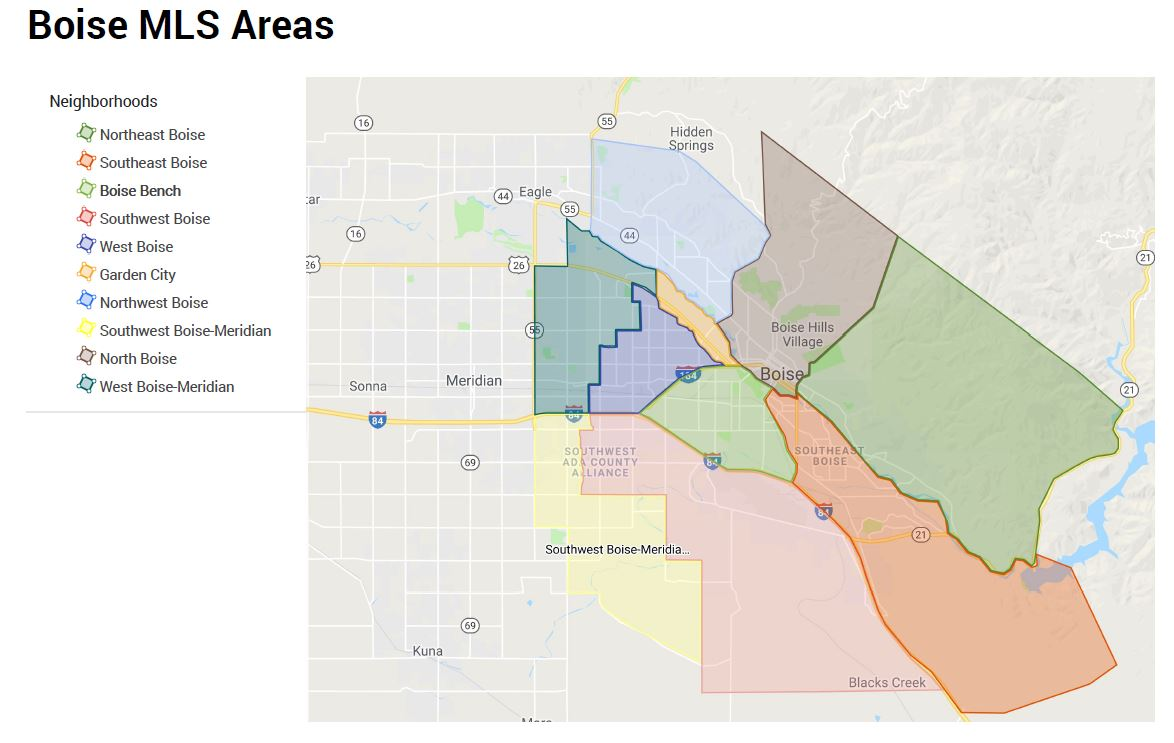
\includegraphics[width= .8\linewidth]{images/MLS_Areas.JPG}
    \caption{MLS Areas of Boise}
    \label{fig: mls_map}
\end{figure}

\begin{table}[H]
    \centering
    \resizebox{.3\textwidth}{!}{
    \begin{tabular}{|l|}
    \Xhline{1 pt}
    \textbf{MLS Area}\\
    \Xhline{1 pt}
    Boise Bench \\
    \Xhline{1 pt}
    Eagle\\
    \Xhline{1 pt}
    Garden City \\
    \Xhline{1 pt}
    North East Boise\\
    \Xhline{1 pt}
    North East Meridian\\
    \Xhline{1 pt}
    North Boise\\
    \Xhline{1 pt}
    North West Boise Garden City\\
    \Xhline{1 pt}
    South East Boise\\
    \Xhline{1 pt}
    South West Boise\\
    \Xhline{1 pt}
    South West Boise Meridian\\
    \Xhline{1 pt}
    West Boise\\
    \Xhline{1 pt}
    West Boise Meridian \\
    \Xhline{1 pt} 
    \end{tabular}}
    \caption{Boise MLS Areas}
    \label{tab: mls_areas}
\end{table}
The housing data needed some cleaning before use. I wanted to find the percent change in value in single family homes from the previous year, I did find that there were some empty lots turned into single family homes that had to be removed, as the change in value was not truly representative.\par
I obtained the jobs data sets from the Bureau of Labor Statistics. This data included a break down by major job category, see Table \ref{tab: job_categories}, and I found the percent change in employment numbers from the previous year. These job categories don't directly correspond to the sectors highlighted by the Brookings report. 



\begin{table}[H]
    \centering
    \resizebox{.8\textwidth}{!}{
    \begin{tabular}{|l|l|}
    \Xhline{1 pt}
    Architecture And Engineering Occupations &Arts, Design, Entertainment, Sports, And Media $\dots$\\
    \Xhline{1 pt} 
    Building And Grounds Cleaning And Maintenance $\dots$& Business And Financial Operations Occupations\\
    \Xhline{1 pt} 
    Community And Social Service Occupations& Computer And Mathematical Occupations\\
    \Xhline{1 pt} 
    Construction And Extraction Occupations&Education, Training, And Library Occupations\\
    \Xhline{1 pt} 
    Farming, Fishing, And Forestry Occupations&
    Food Preparation And Serving Related Occupations\\
    \Xhline{1 pt} 
    Healthcare Practitioner And Technical Occupations&
    Healthcare Support Occupations\\
    \Xhline{1 pt} 
    Installation, Maintenance, And Repair Occupations&
    Legal Occupations\\
    \Xhline{1 pt} 
    Life, Physical, And Social Science Occupations&
    Management Occupations\\
    \Xhline{1 pt} 
    Office And Administrative Support Occupations&
    Personal Care And Service Occupations\\
    \Xhline{1 pt} 
    Production Occupations&
    Protective Service Occupations\\
    \Xhline{1 pt} 
    Sales And Related Occupations&
    Transportation And Material Moving Occupations\\
    \Xhline{1 pt} 
    \end{tabular}}
    \caption{Major Job Categories}
    \label{tab: job_categories}
\end{table}







\section{Methods}

\paragraph{}I initially developed the model with all of the job categories listed in Table \ref{tab: job_categories}. I the checked the Variance Inflation Factor (VIF) of the model. The VIF is used in regression analysis to assess the collinearity between the predictors, if the result is close to 1 it is good, but if the result is greater than 10 then it shows high multicollinearity. I found that the VIF score was essentially infinite which meant that I could not use the model as it was. I was then advised to perform an Automated Stepwise Regression on the data to see which of the variables I could use. I followed the steps in the Book "Statistical Analysis and Data Display An Intermediate Course with Examples in R" By Richard M. Heiberger and Burt Holland, page 297-311. When I ran the Stepwise Regression the best predictors found can be seen in Table \ref{tab: feature_key}. I then relabeled the job categories for ease of reading in plots.

\begin{figure}[H]
    \centering
    \begin{subfigure}[b]{.3\linewidth}
    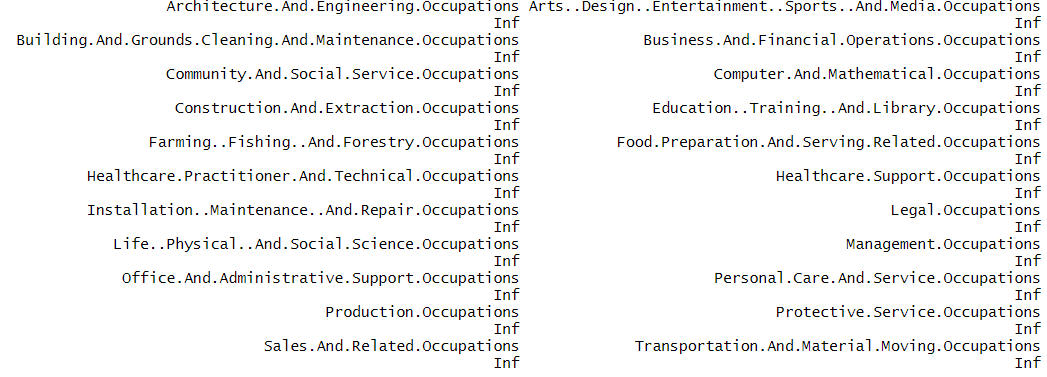
\includegraphics[width =\linewidth]{images/InfVif.PNG}
    \caption{VIF for All Job Categories}
    \label{fig:infVif}
    \end{subfigure}
    \begin{subfigure}[b]{.6\linewidth}
    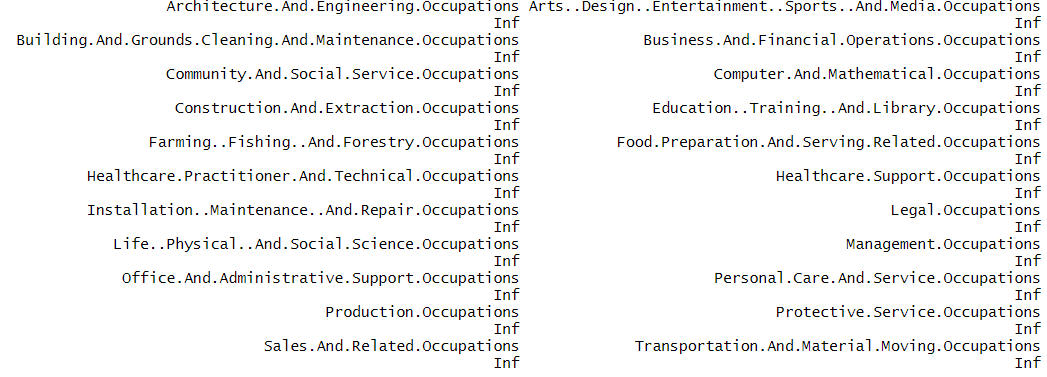
\includegraphics[width =\linewidth]{images/InfVif.PNG}
    \caption{VIF with Best Model}
    \label{fig:bestVIF}
    \end{subfigure}
    \caption{Variance Inflation Factor (VIF)}
    \label{fig:vif}
\end{figure}

\begin{table}[H]
    \centering
    \resizebox{.6\textwidth}{!}{
    \begin{tabular}{|c|l|}
    \Xhline{1 pt}
    \textbf{Key}&\textbf{Feature Name}\\
    \Xhline{1 pt}
    Job 1     &  Arts, Design, Entertainment, Sports, And Media...\\
    \Xhline{1 pt} 
    Job 2  &  Education, Training, And Library Occupations\\
    \Xhline{1 pt} 
    Job 3  &  Farming, Fishing, And Forestry Occupations\\
    \Xhline{1 pt} 
    Job 4  &  Food Preparation And Serving Related Occupations\\
    \Xhline{1 pt} 
    Job 5  & Life, Physical, And Social Science Occupations\\
    \Xhline{1 pt} 
    Job 6  &  Management Occupations\\
    \Xhline{1 pt} 
    Job 7  & Personal Care And Service Occupations\\
    \Xhline{1 pt} 
    Job 8  & Production Occupations\\
    \Xhline{1 pt} 
    \end{tabular}}
    \caption{Feature Key Table}
    \label{tab: feature_key}
\end{table}

I then ran the VIF test as well as checking the residuals

\begin{figure}[H]
    \centering
    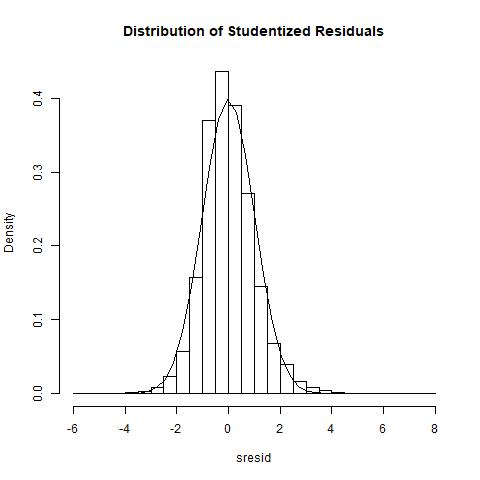
\includegraphics[width= .6\linewidth]{images/student_resid_plot.jpeg}
    \caption{Studentized Residuals}
    \label{fig: student_resid}
\end{figure}

\begin{figure}[H]
    \centering
    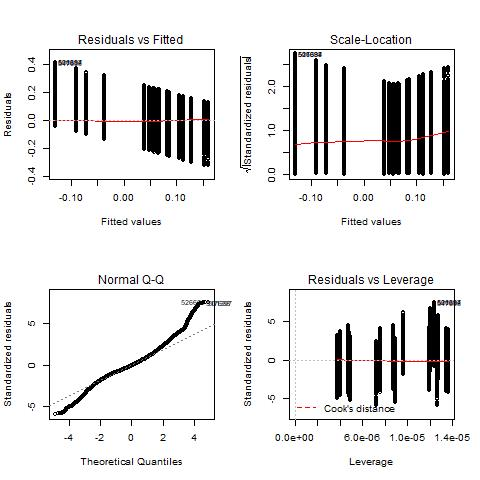
\includegraphics[width= .8\linewidth]{images/plot_matrix.jpeg}
    \caption{Plots of Tests of the Model}
    \label{fig: plot_matrix}
\end{figure}



\section{Results}










\begin{figure}[H]
    \centering
    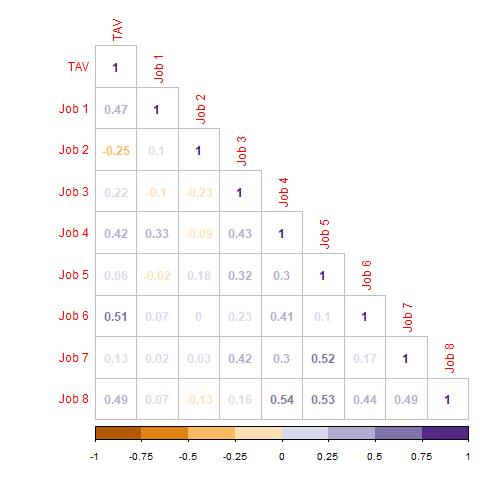
\includegraphics[width=.6\linewidth]{images/corr_matrix.jpeg}
    \caption{Correlation Matrix}
    \label{fig:corrMatrix}
\end{figure}

\begin{table}[H]
    \centering
    \resizebox{.95\textwidth}{!}{
    \begin{tabular}{|l|c|c|c|c|c|c|c|c|}
    \Xhline{1pt}
     MLS Area & Job 1 & Job 2 & Job 3 & Job 4&Job 5&Job 6&Job 7&Job 8 \\
     \Xhline{1.5 pt}
     All of Boise &0.47244 &-0.25452& 0.22131& 0.42181&0.05528& \cellcolor{yellow}0.51403& 0.13477& 0.49349\\
     \Xhline{1.5 pt}
    Boise Bench & 0.37016 &-0.18183 &0.18004& 0.32748& 0.07605&\cellcolor{yellow} 0.47899& 0.15502 &0.47829\\
    \Xhline{1 pt}
    Eagle&0.27020& -0.23780& 0.18223 &0.38202&0.18830 &0.45410& 0.16035&\cellcolor{yellow} 0.48101\\
    \Xhline{1 pt}
    Garden City & 0.47347 &-0.16628& 0.12171& 0.39270 &-0.01083& \cellcolor{yellow}0.54356& 0.05221& 0.35181\\
    \Xhline{1 pt}
    North East Boise &0.44502 &-0.30788 &0.31044 &0.44801 &0.11171 &\cellcolor{yellow} 0.52445 &0.14307& 0.45781\\
    \Xhline{1 pt}
    North East Meridian& 0.51055 & -0.22300 &0.22524 &0.50716 & -0.08835 & \cellcolor{yellow} 0.60318 & 0.09026& 0.53070\\
    \Xhline{1 pt}
    North Boise&0.41560 &-0.35709& 0.31848& 0.39945& -0.01637& \cellcolor{yellow}0.49233& 0.09699 &0.37526\\
    \Xhline{1 pt}
    North West Boise-Garden City& \cellcolor{yellow}0.52669 & -0.25098 & 0.15905 & 0.40713& 0.06458 &0.51001& 0.15309 &0.49626\\
    \Xhline{1 pt}
    South East Boise& 0.50898& -0.25805& 0.23049&0.42712& 0.07212 & \cellcolor{yellow}0.54420 & 0.10922 &0.50249 \\
    \Xhline{1 pt}
    South West Boise& \cellcolor{yellow}0.62526 &-0.32890& 0.30176 & 0.57181 & 0.14149 & 0.57526 & 0.13010 & 0.61330\\
    \Xhline{1 pt}
    South West Boise Meridian& \cellcolor{yellow}0.57333 & -0.23180 & 0.25831 & 0.56873 & 0.05242 &0.54541 & 0.16347& 0.57175\\
    \Xhline{1 pt}
    West Boise&0.49497 &-0.24963&  0.17686& 0.42427& 0.07121 & 0.50468 &0.14486 &\cellcolor{yellow}0.52594\\
    \Xhline{1 pt}
    West Boise Meridian& 0.49958 &-0.23565& 0.20646& 0.47795& 0.04509 &0.51593& 0.16244 &\cellcolor{yellow}0.55835 \\
    \Xhline{1 pt} 
    \end{tabular}}
    \caption{Correlation Coefficients by MLS Area}
    \label{tab:my_label}
\end{table}


\section{Comments and Conclusions}
\paragraph{}I was surprised that Management Occupations was the greatest influence on the TAV of my home in the Boise Bench. I was expecting it to be Computer and Mathematical Occupations, but the computer occupations did not make it through the stepwise regression. Further research could dig further into the details of each job category and how the salary increases of that category played into the changes in housing prices. Also the stepwise regression could be run against each MLS area individually to see if there are different occupations that make it through the stepwise regression other than the occupations listed in Table \ref{tab: feature_key}.


\newpage

\section*{Appendix A}\label{appendixA}
\subsection{Description of Job Categories}
\begin{enumerate}
    \item Arts, Design, Entertainment, Sports, And Media
        \begin{itemize}
            \item Art and Design Workers
            \item Entertainers and Performers, Sports and Related Workers
            \item Medial and Communication Workers
        \end{itemize}
    \item  Education, Training, And Library Occupations
        \begin{itemize}
            \item Teachers, all levels
            \item Librarians, Curators, and Archivists
            \item Instructors
        \end{itemize}
    \item  Farming, Fishing, And Forestry Occupations
        \begin{itemize}
            \item  Agricultural Workers
            \item Fishing and Hunting Workers
            \item Forest and Conservation Workers
        \end{itemize}
    \item  Food Preparation And Serving Related Occupations
        \begin{itemize}
            \item Supervisors of Food Preparation and Serving Related Workers
            \item Cooks and Food Preparation Workers
            \item Food and Beverage Serving Workers
            \item Other Food Preparation and Serving Related Workers
        \end{itemize}
    \item  Life, Physical, And Social Science Occupations
        \begin{itemize}
            \item Life Scientists
            \item Physical Scientists
            \item Social Scientists and Related Workers
        \end{itemize}
    \item  Management Occupations
        \begin{itemize}
            \item Top Executives
            \item Advertising, Marketing, Promotion, Public Relations, and Sales Managers
            \item Operations Specialities Managers
            \item All other Managers
        \end{itemize}
    \item  Personal Care And Service Occupations
        \begin{itemize}
            \item Supervisors of Personal Care Workers
            \item Animal Care and Service Workers
            \item Entertainment Attendants and Related Workers
            \item Funeral Service Workers
            \item Personal Appearance Workers
            \item Tour and Travel Guides
            \item Other Personal Care Workers
        \end{itemize}
    \item  Production Occupations
        \begin{itemize}
            \item Supervisors of Production Workers
            \item Assemblers and Fabricators
            \item Food Processing Workers
            \item Metal and Plastic Workers
            \item Woodworkers
            \item Plant and System Operators
        \end{itemize}
\end{enumerate}
\newpage
%------------------------------------------------------------------------------%
% References
%------------------------------------------------------------------------------%
\begin{thebibliography}{3}

\bibitem[\protect\astroncite{ACAO}{2019}]{ACAO:2019}
Ada County Assessor's Office (July 8, 2019)
\newblock \textit{Residential House Details for homes in Boise Idaho, from 2000-July 8, 2019}.
% Compiled by Alan Smith Strategic Development Analyst
%\newblock 


\bibitem[\protect\astroncite{KWR}{2019}]{KWR:2019}
Keller Williams Reality Boise (August 6, 2019)
\newblock \textit{Boise Neighborhood Guide}.
\newblock \url{https://www.weknowboise.com/boise-neighborhoods.php}




\bibitem[\protect\astroncite{ESCO}{2019}]{ESCO:2008}
Escobari, Marcela; Seyal, Ian; Morales-Arilla Jose;and Shearer, Chad (2019)
\newblock Growing Cities that Work for All
\newblock \textit{Brookings}.

\bibitem[\protect\astroncite{Heiberger and Holland}{2009}]{Heiberger:Holland:200p}
Heiberger, R. and Holland, B. (2008)
\newblock 
\newblock \textit{Journal of the American Statistical AssociationStatistical Analysis and Data Display: An Intermediate Course with Examples in R}, 297-313.


\bibitem[\protect\astroncite{BLS}{2019}]{BLS:2019}
United States Bureau of Labor Statistics (August 3, 2019)
\newblock \textit{Occupational Employment Statistics}.
% Last Modified Date: March 29, 2019
\newblock \url{https://www.bls.gov/oes/tables.htm}

\bibitem[\protect\astroncite{USC}{2019}]{USCB:2019}
United States Census Bureau, Population Division (August 4, 2019)
\newblock \textit{Annual Estimates of Housing Units for the United States, Regions, Divisions, States, and Counties: April 1, 2010 to July 1, 2018 Release Date: May 2019}.
% https://factfinder.census.gov/faces/tableservices/jsf/pages/productview.xhtml?pid=PEP_2018_PEPANNHU&prodType=table
%\newblock \url{https://www.bls.gov/oes/tables.htm}
%https://www.census.gov/data/tables/time-series/demo/popest/intercensal-2000-2010-housing-units.html


%https://www.ktvb.com/article/news/wall-street-journal-notes-red-hot-boise-housing-market/277-bf82d25c-334b-432c-ace6-7480dd3f5c86



% \bibitem[\protect\astroncite{Chen and Wu}{2008}]{Chen:Wu:2008}
% Chen, J. and Wu, H. (2008)
% \newblock Efficient local estimation for time-varying coefficients in
% deterministic dynamic models with applications to {HIV}-1 dynamics.
% \newblock \textit{Journal of the American Statistical Association}, 103, 369--384.

% \bibitem[\protect\astroncite{Shumway and Stoffer}{2011}]{Shumway:Stoffer:2011}
% Shumway, R. H. and Stoffer, D. S. (2011)
% \newblock \textit{Time Series analysis and Its Applications With R Examples}, 3rd edn.
% \newblock New York: Springer.
\end{thebibliography}
%-----------------------------------------------------------------------------%
\end{document}
%-----------------------------------------------------------------------------%
    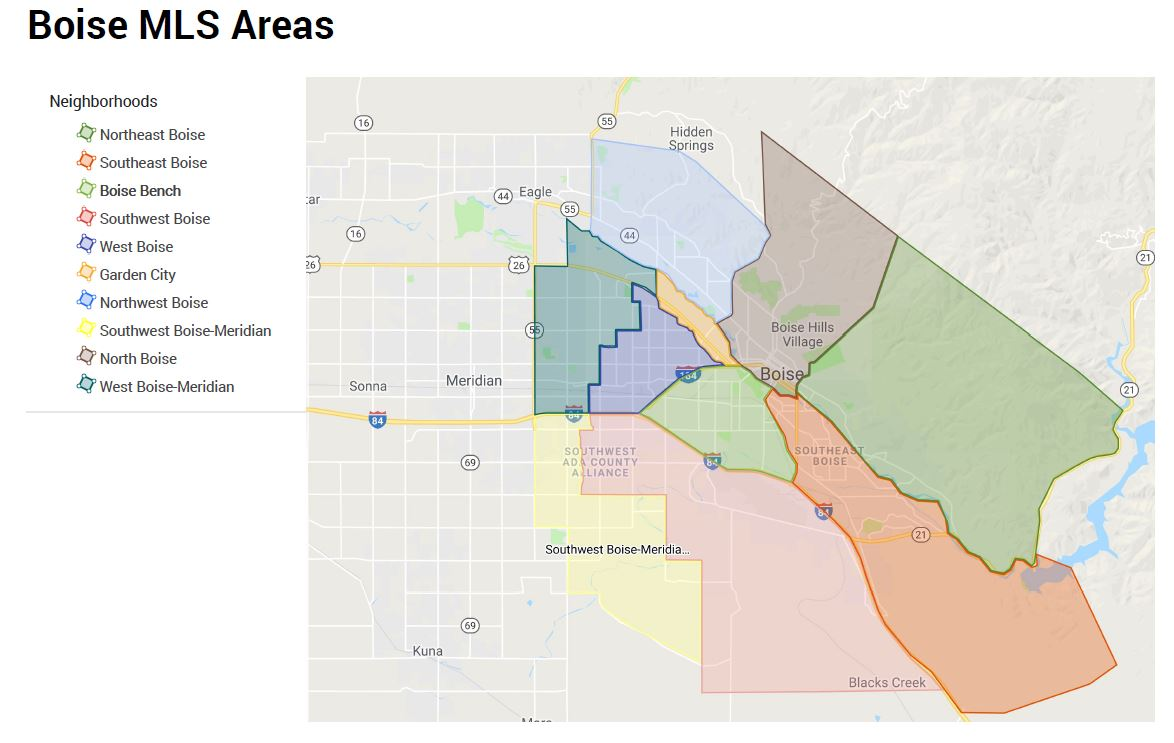
\includegraphics[width= .7\linewidth]{images/MLS_Areas.JPG}

